\documentclass{article}
\usepackage{amsmath}
\usepackage{amssymb}
\usepackage{array}
\usepackage{booktabs}
\usepackage{makecell}
\usepackage{multirow}
\usepackage{enumitem}
\usepackage{diagbox}
\usepackage{tabularx}
\usepackage{graphicx}
% \usepackage[top=3cm,bottom=2cm,left=2cm,right=2cm]{geometry} % 页边距
\title{Software System Design-Architecture\\Assignment 3\\C4 System Architecture Design}
\author{4 people}

\begin{document}
	\maketitle
	\newpage
	\section{Deploying ADD method in C4 Design}
	\subsection{Important Non-functional Requirements}
	The important non-functional requirements we identified are listed bellow:
	\begin{itemize}
		\item {Availability}
		\item {Performance}
		\item {Modification}
		\item {Scalability}
		\item {Interoperability}
		\item {Consistancy}
		\item {Integrity}
		\item {Usability}
	\end{itemize}
	The constrains we identified are listed bellow:

	\begin{itemize}
		\item No persistent data caching on the agent workstations to limit the implications of local failures.
		\item No DBs at office locations.
		\item No administrators at local offices.
		\item No maintenance down-time.
		\item The middle layer server cluster tuned for performance.
		\item The back end tuned for DB performance.
		\item Well engineered operations architecture.
		\item High availability cannot be achieved by utilizing fault-tolerant hardware (this option is not
		economically viable).
	\end{itemize}
	The scenarios are listed as following:

	\begin{center}
		\begin{table}[!htb]
		\begin{tabular}{ccc}
		\toprule  
		Portion of Scenario & Possible Values\\
		\midrule 
		Source & End users and internal systems.\\
		Stimulus & Failure and fault: Service off-line, error, \\
		& crash ans so on.\\
		Artifact & Back up, spare, communication channels.\\
		Environment & Runtime, startup and shutdown, in-service.\\
		Response & Able to response for many requests at the \\
		& same time.\\
		& Detect the fault. \\
		& Recover from the fault. \\
		& Prevent the fault. \\		
		Response Measure & Availability percentage(e.g. 99\%) \\
		& Time to be back to service after an error occured \\
		& Time to detect a failure \\
		\bottomrule
		\end{tabular}
		\caption{Availability Scenario}
		\end{table}
	\end{center}

	\begin{center}
		\begin{table}[!htb]
		\begin{tabular}{ccc}
		\toprule  
		Portion of Scenario & Possible Values\\
		\midrule 
		Source & End users and internal systems.\\
		Stimulus & Many requests come at the same time.\\
		Artifact & A waiting queue or something could  \\
		& caching the request temporarily. A mechanism  \\
		& to serve the request after a short interval.\\
		Environment & In-service. \\
		Response & The C4 should be able to deal with a large \\
		& bunchs of requests. And after a short interval, the \\
		& request would be processed.\\
		Response Measure & The time taken to serve every request.\\
		& The lateness of the processing.\\
		\bottomrule
		\end{tabular}
		\caption{Performance Scenario}
		\end{table}
	\end{center}

	\begin{center}
		\begin{table}[!htb]
		\begin{tabular}{ccc}
		\toprule  
		Portion of Scenario & Possible Values\\
		\midrule 
		Source & Developers.\\
		Stimulus & Add some interface to fit for a new requirement.\\
		& Need to improve the system to cater for the increasing \\
		& demand resulted from the rapid growing users.\\
		Artifact & Code, interface, components and so on.\\
		Environment & Runtime or off-line, in the design \\
		& process or in the maintaining process\\
		Response & Make the modifications.\\
		Response Measure & The effort, time and money taken\\
		& to implement such requirement.\\
		\bottomrule
		\end{tabular}
		\caption{Modification Scenario}
		\end{table}
	\end{center}


	\begin{center}
		\begin{table}[!htb]
		\begin{tabular}{ccc}
		\toprule  
		Portion of Scenario & Possible Values\\
		\midrule 
		Source 				& The client is going to request related infomation \\
							& from the target server , usually the important \\
							& personal infomation\\
		Stimulus 			& The infomation sends back to the client\\
		Artifact 			& Client PC	\\
		Environment 		& Query from DB , server cache and Request queue\\
		Response 			& The server has to fetch the user request and \\
							& conduct the related query from the data source , \\
							& with the maintainance of the data integrity. \\
							& To maintain the data integrity , the server \\
							& should checkout whether the data has the \\
							& lattest version and no other conflict \\
							& writing conduction is on going.\\
		Response Measure 	& The data sent back to the user\\
							& has to be 100 percents integrity.\\

		\bottomrule
		\end{tabular}
		\caption{Integrity Scenario}
		\end{table}
	\end{center}
	
	\begin{center}
		\begin{table}[!htb]
		\begin{tabular}{ccc}
		\toprule  
		Portion of Scenario & Possible Values\\
		\midrule 
		Source 				& More customer load push on the system\\
		Stimulus 			& More than five thousand of user are using the system\\
		Artifact 			& Master server , keeper\\
		Environment 		& Network connection , agent requests \\
		Response 			& The server should detect the specific \\
							& server that is overloadded, \\
							& and reallocate the request to other leisure node;\\
							& The keeper should arrange the request queue to ensure \\
							& the syncronize the data flow in the process ,\\
							& ensuring the data is always correct.\\
		Response Measure 	& Load balance , horizontal expansion and reqeust queue \\
							& to resolve the high concurrency\\


		\bottomrule
		\end{tabular}
		\caption{Availability Scenario}
		\end{table}
	\end{center}

	\begin{center}
		\begin{table}[!htb]
		\begin{tabular}{ccc}
		\toprule  
		Portion of Scenario & Possible Values\\
		\midrule 
		Source 				& One agent somhow choose to save the session and \\
							& return back to continue the session.\\
		Stimulus 			& The system is going to save the context of the \\
							& current session of agents.\\
		Artifact 			& A session which represents the current \\
							& state of both agents' infomation , \\
							& session attributes and so on.\\
		Environment 		& keeper \\
		Response 			& The keeper reply the saving request \\
							& and put the session infomation to the \\
							& base storage in keeper's cluster , \\
							& and set back the session identification to agents.\\
		Response Measure 	& Set up local storages which is reponsible of saving sessions\\
							&  in the server of keeper and  \\
							& arrange the location of the storage.\\
		\bottomrule
		\end{tabular}
		\caption{Usability Scenario}
		\end{table}
	\end{center}

	\subsection{Records of ADD iterations}
		\subsubsection{Iteration 1}
		Chosen element: the whole system.
		Chosen ASR: 
		1. near 7x24 availability.
		2. It should allow for "leaner" growth and should be able to grow at a rapid rate.
		Design Concerns: high  availability, high scalability.
		Candidate architecture patterns:\\

		\begin{tabular}{|c|c|c|}
			\hline
			pattern name & complexity& fault-tolerance\\
			\hline
			broker& low& low\\
			\hline
			redundant broker& high& high\\
			\hline
		\end{tabular}
		\\\\
		Chosen pattern: redundant broker
		Reason: Added broker can help manage server nodes and easily achieve high availability. But the business background goal that the system can handle requests simultaneously with highly growing customers will implies high pressure on the broker. Redundant broker is adopted for data back-up quick switch in emergency condition. 

		\subsubsection{Iteration 2}
		Chosen element: master.
		Chosen ASR: 
		1.can handle a batch of requests simultaneously and can support multiple agents.
		2.should manage a big cluster/allow for "leaner" growth
		3.near 7x24 availability.
		4.identification, monitoring, and elimination of processing bottle-necks
		Design Concerns:
		Master Self-test
		Real-time Server Detection:Health detection
		Server Recovery: Fast restart, Transparency to PC, Data recovery
		Service Registry: Locating nodes, Resource allocation, Resource collection, Horizontal extension

		Candidate architecture patterns/tactics:
		Master Self-test:
			pattern name, detection latency
			Hot spare, <100ms
			Warm spare, >1s
			Cold spare, >5s

		Health detection:
			pattern name, communication pressure, storage pressure, report threshold, rate, transparent to PC
			Loading table, high, high, no, controllable, yes 
			Server warning, low, low, controllable, up to context, almost
			PC warning, no, no, uncontrollable, up to context, not
		
		Fast restart:
			...
		
		Transparency to PC:
			...
		
		Data Recovery:
			...
		
		Service Registry:
			...
		
		Locating nodes:
			... 

		Resource allocation:
			...

		Resource collection:
			... 

		Horizontal extension:
			...

		Chosen pattern/tactics:
			Master Self-test:
				Hot spare
			Chosen reason: 

			Health detection:
				Loading table
			
			Fast restart:
				
			
			Transparency to PC:
				...
			
			Data Recovery:
				...
			
			Service Registry:
				...
			
			Locating nodes:
				... 

			Resource allocation:
				...

			Resource collection:
				... 

			Horizontal extension:
				...
		

	\section{Final Software Architecture Documentation}
	\subsection{Documentation Roadmap}
	\subsubsection{Scope and summary}
	This documentation is built for presence, explanation and analysis of the architecture of Call Center Customer Care(C4) System, which will be employed by ** US telecommunication company. In this documentation, expression and illustration of modules and theirs relationship will be covered, but not all functions of the system are included.
	\subsubsection{How the documentation is organized}
	cateloge
	\subsubsection{View overview}
	4 Views are employed to illustrate the architecture, including:\\  
	Decomposition view: The elements of this view are static modules, and connections illustrate their relationship.\\  
	Shared-data view: We using this view to express how important data are shared and protected from inconsistency resulted by business events....  \\
	Deployment view: This view also illustrate different parts of the software. Distinguished with module view, it focuses on the runtime status rather than the static status of the system.\\
	All of the three views are following the standard UML specification.
	\subsubsection{How stakeholders can use this documentation}
	Use for specification, evaluation, development, test, deployment.

	\subsection{How a View Is Documented}
	Refer to the view template

	\subsection{System Overview}
	System functions, users, important background, constrains.
	
	\subsection{Views}
		\subsubsection{Decomposition View} 
			\paragraph{Section 1: The Primary Presentation}
			\begin{center}
			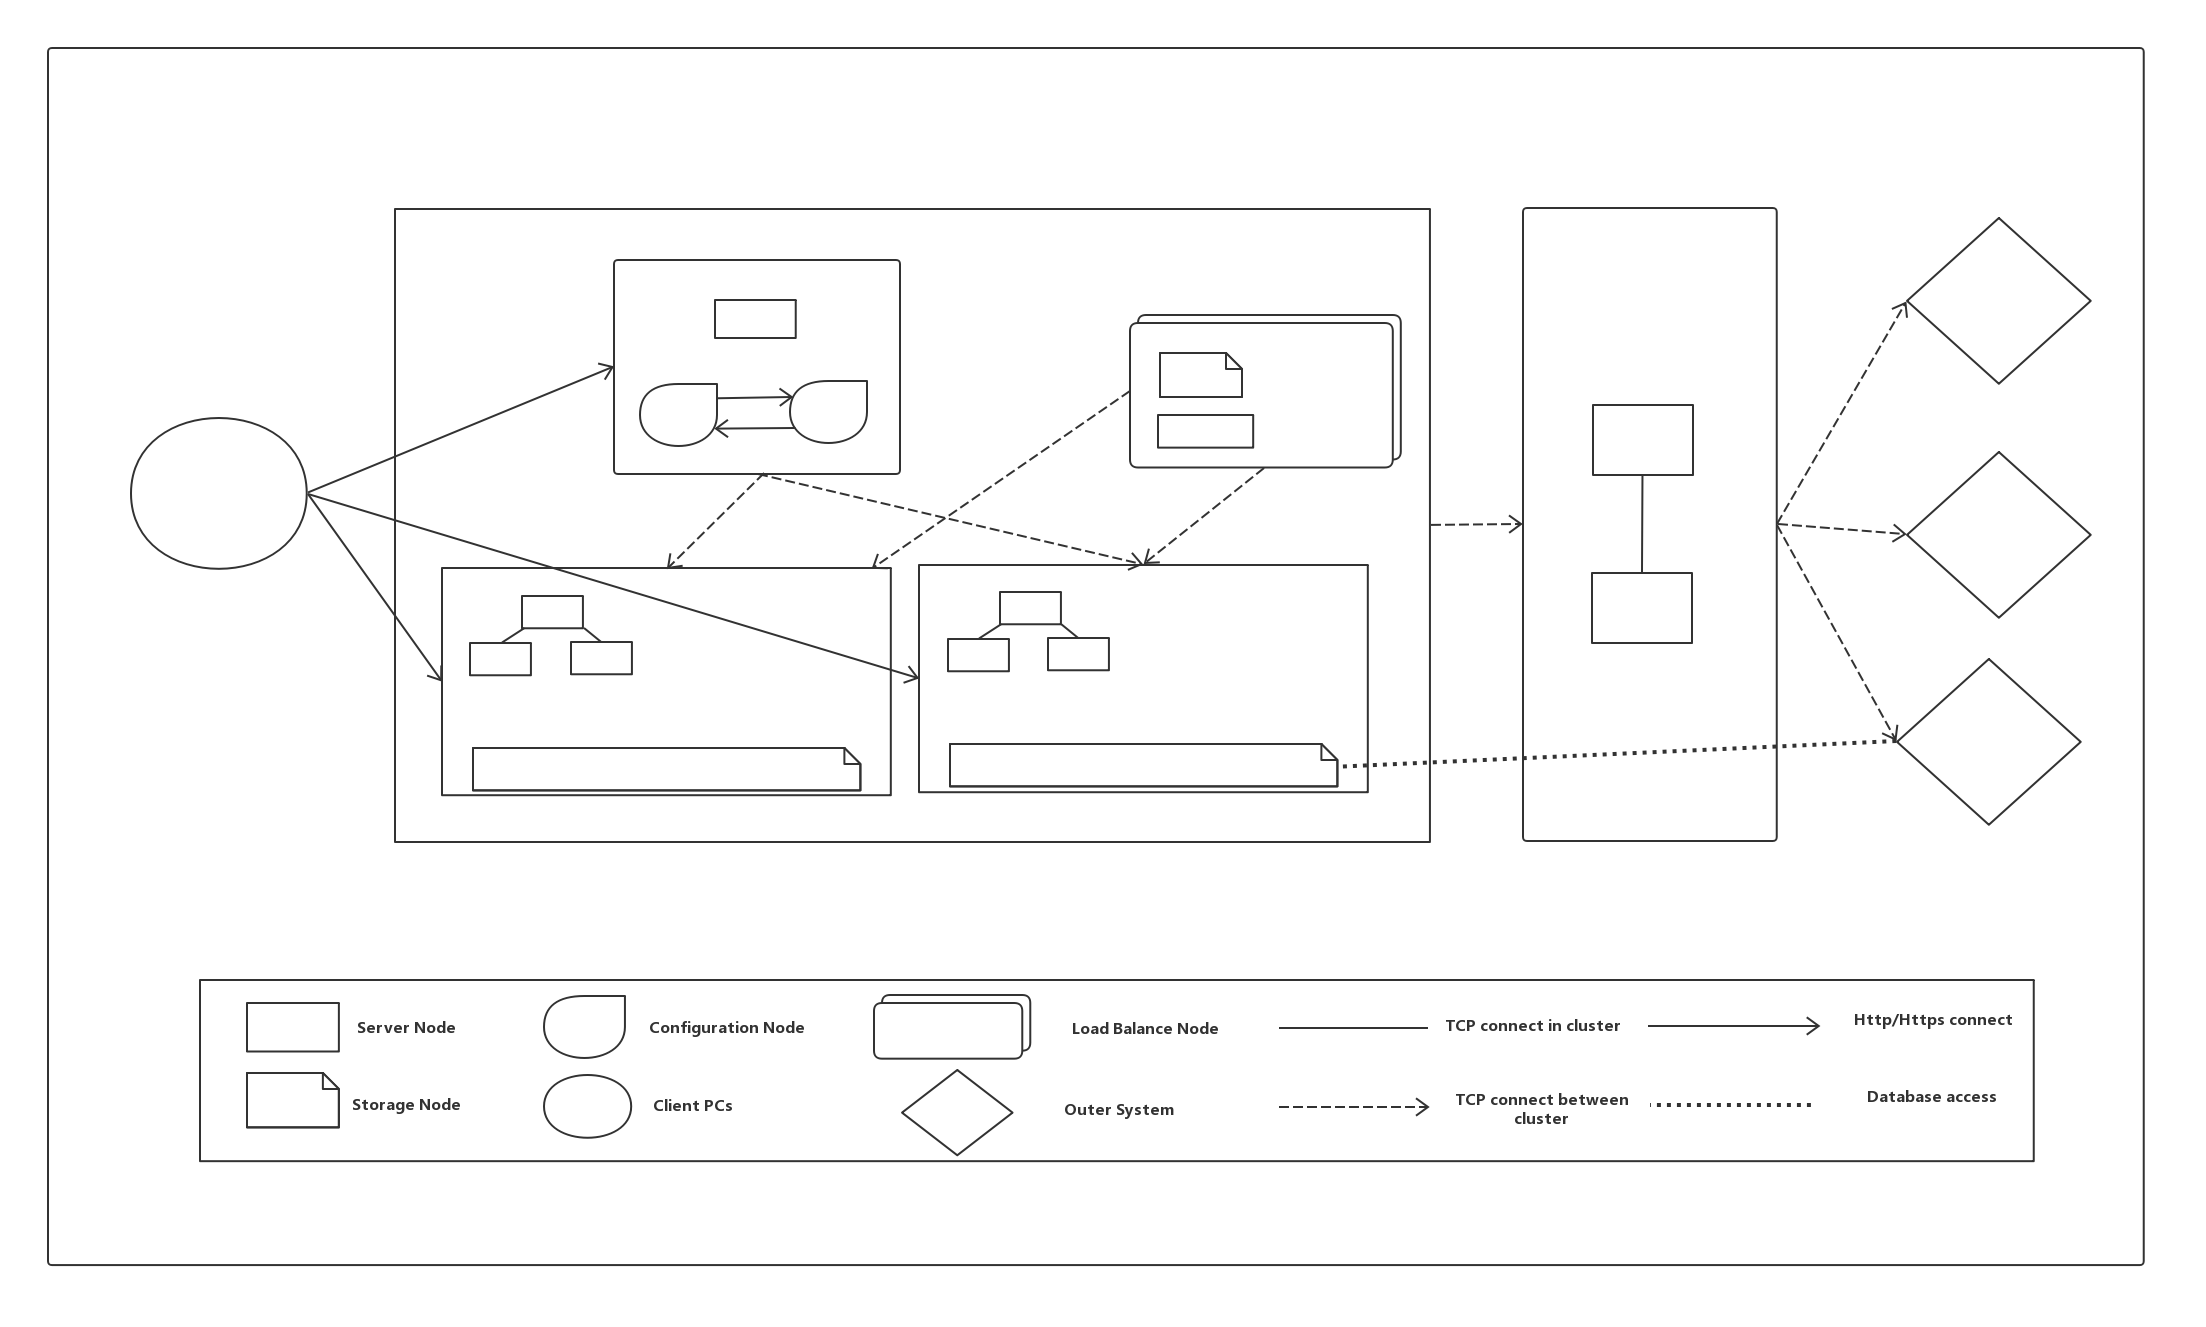
\includegraphics[scale=0.15]{decom_section1.png}
			\end{center}
			\paragraph{Section 2: The Element Catalog}
			The C4 system is consisted of these important sub-module to decompose:  master node , normal server node , storage node , configuration node , load balance node. To resolve the normal phone request (contains the sync-request and async-request) , the normal server nodes are responsible to tackle the service from customers. Moreover , the storage nodes have to save the current session , cache the query on DB , and other cache to the locks . Load balance node has to detect the load in the whole system , and reschedule the load accordingly. 
			\paragraph{Section 3: Context Diagram}
			\begin{center}
			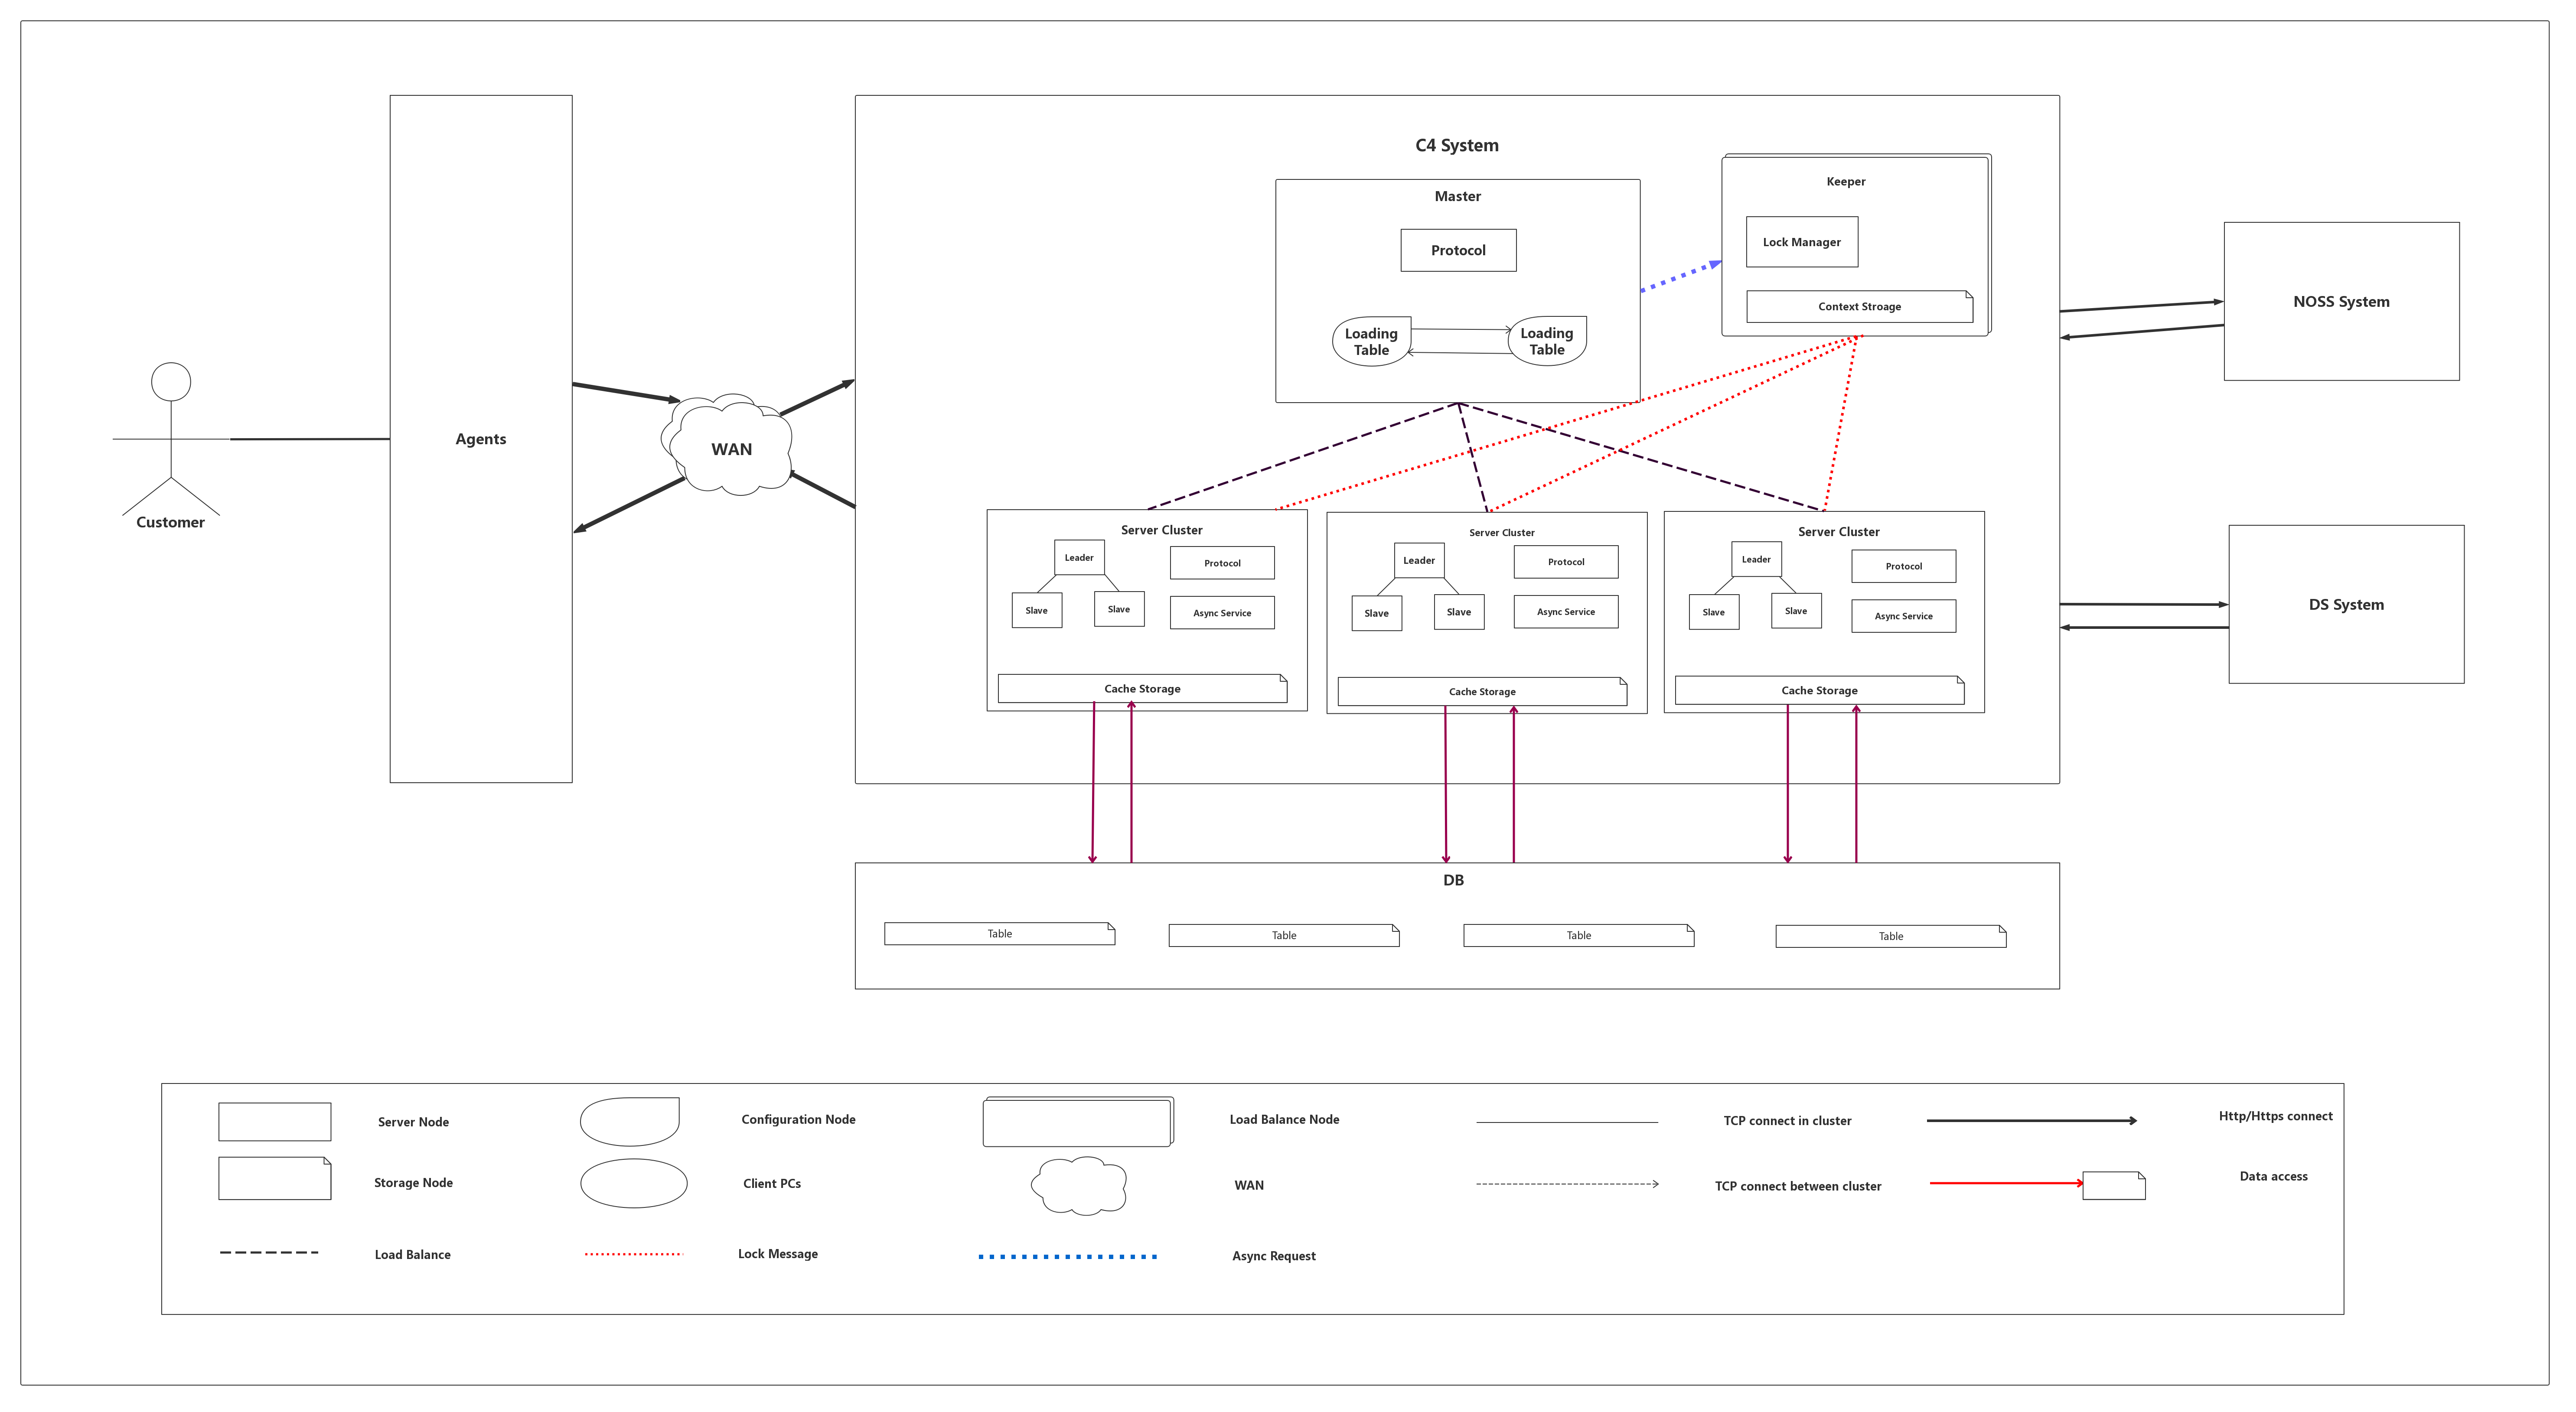
\includegraphics[scale=0.05]{decom_section2.png}
			\end{center}
			\paragraph{Section 4: Variability Guide}
			The decomposition view represents the template module in the C4 system , and to exercise the variation points , you are recommended to run the server node. With the sync-request (like fetching user basic information , setting up a new session)  and async-request (conflict between the different sessions) , you could catch the key points in the master.
			\paragraph{Section 5: Rationale}
			The PC agents communicate with C4 system across the WAN. 
			Master node stands for the whole manager of C4 system . That is ,  the master node uses the loading table to temporarily record the load status of all subordinate slave server clusters, and can timely alarm and resource reallocation. The master node also contains a protocol subnode, which is mainly used to help the master node process user requests. After the agents send the request, they will first be parsed by the master node to inform the agents of the required service node location, and then the agents will send the request to the target server.	
			The keeper is responsible for asynchronous event processing and session saving between server nodes. Use Lock Manager to allocate locks and save contexts through context storage.
			The server node is mainly responsible for periodically reporting heart beat status to the master node, and can perform hot backup between nodes. Please note that one server node here is also a cluster. In our design, one cluster is responsible for a certain range. The service (similar to the microservices architecture), and the leader is elected by the vote inside the cluster to perform resource scheduling and service allocation to the subordinate slave. In addition, the server node also supports the processing of the protocol and async service. Responsible for the interaction of the NOSS and DS systems. The cache storage is responsible for the caching of the external DB system. Since each business request will design a query of more than a dozen data tables, considering the time loss of the cascaded query, we use the cache mechanism to The query result is cached inside the server.

		\subsubsection{Shared-Data View} 
			\paragraph{Section 1: The Primary Presentation}
			\begin{center}
			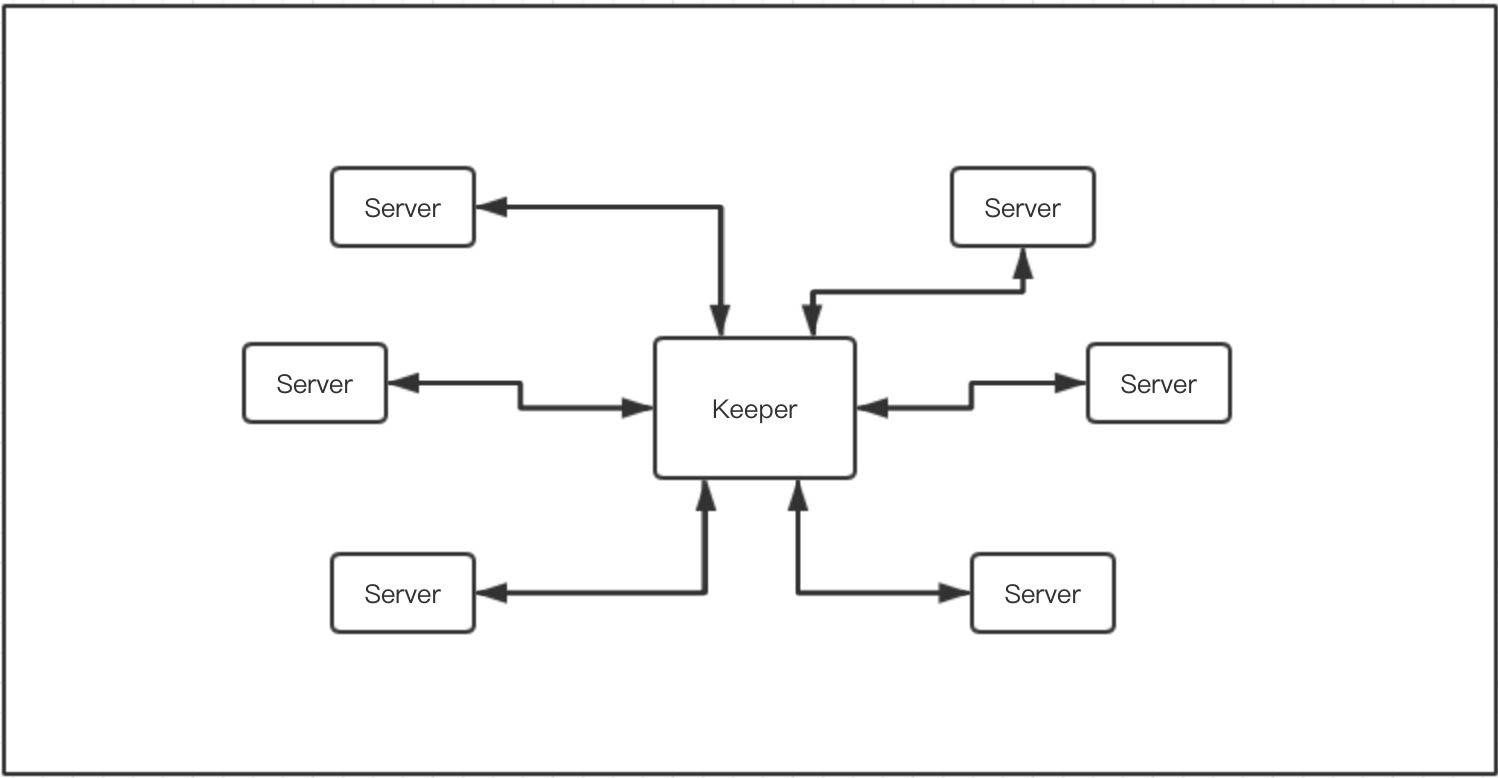
\includegraphics[scale=0.3]{share.png}
			\end{center}
			\paragraph{Section 2: The Element Catalog}
			\subparagraph{Elements and their properties}
			\begin{itemize}
			\item{Keeper} The keeper is a data storage center which holds the shared data.
			\item{Server} The server is an entity which stores and fetches data from the Keeper. For example, when a customer temporarily terminates the process, server should save the context for a future reference.
			\end{itemize}
			\subparagraph{Relations and their properties}
			During the fetching process, there may not exist the record, so there should be an exception. Also, in the saving process, to those records that already existed, saving process should be an update to the old version.
			\subparagraph{Element interfaces}
			The Keeper should provide the find and insert interfaces to the servers.
			\subparagraph{Element behavior}
			The servers save and fetch the data from the Keeper.
			\paragraph{Section 3: Context Diagram}
			\begin{center}
			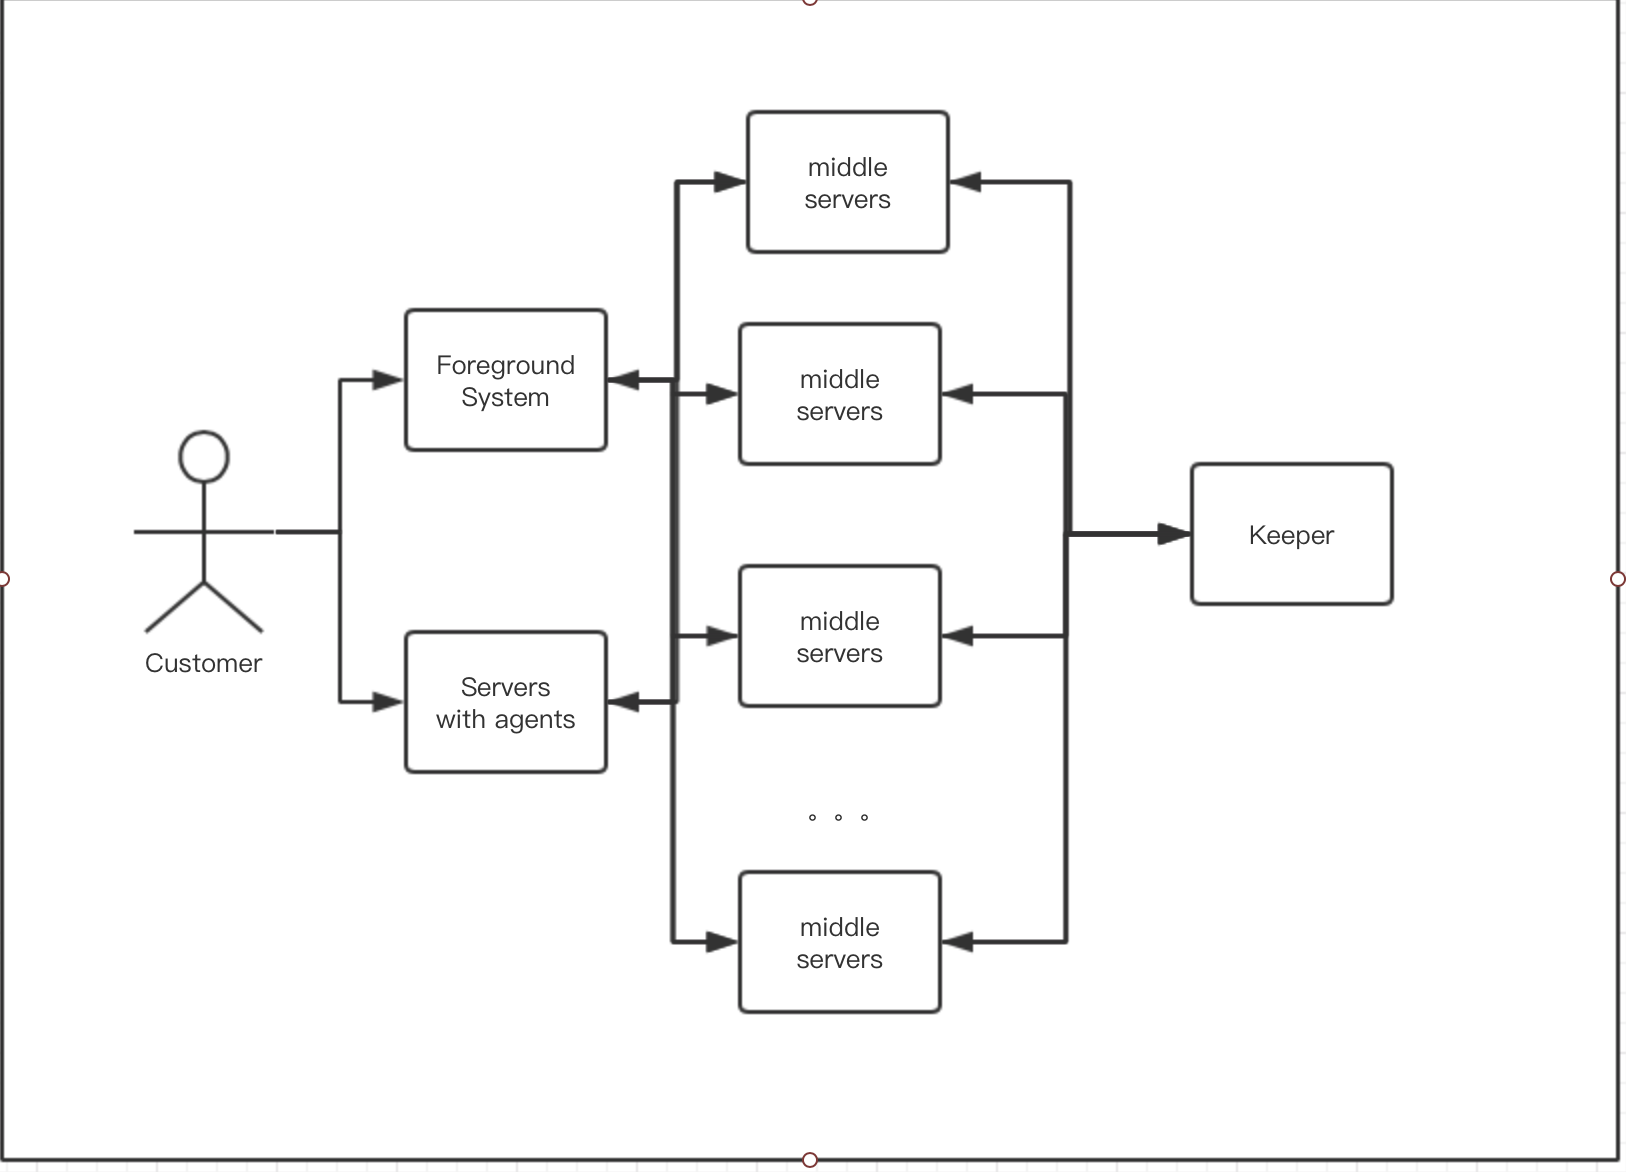
\includegraphics[scale=0.3]{share2.png}
			\end{center}
			\paragraph{Section 4: Variability Guide}
			Because the data storage is not the only responsibility keeper takes, so in the future, it may be  divided into several more specific components, that is to say, the keeper in this view may be changed to a data repository or other data center.
			\paragraph{Section 5: Rationale}
			The design problem came from the requirement "A customer can be interrupted (for technical reasons, for example) or suspended by the customer or the representative ... In any case, C4 has to manage the context that persists and can be recalled."
			In order to do this, there should be a mechanism that stores and fetches the context. There are several options. For example, we can save the information in the agent's PC, or save in the DB provided by the third party. But both of them are infeasible. There is no persistent data caching on the agent workstations, and DB may not be changed since it is provided by the third party. So finally, we choose to save the information in the Keeper, as it is also used to synchronize the event and resolve the conflict as mentioned in the sections before.

		\subsubsection{Deployment View} 
			\paragraph{Section 1: The Primary Presentation}
			\begin{center}
			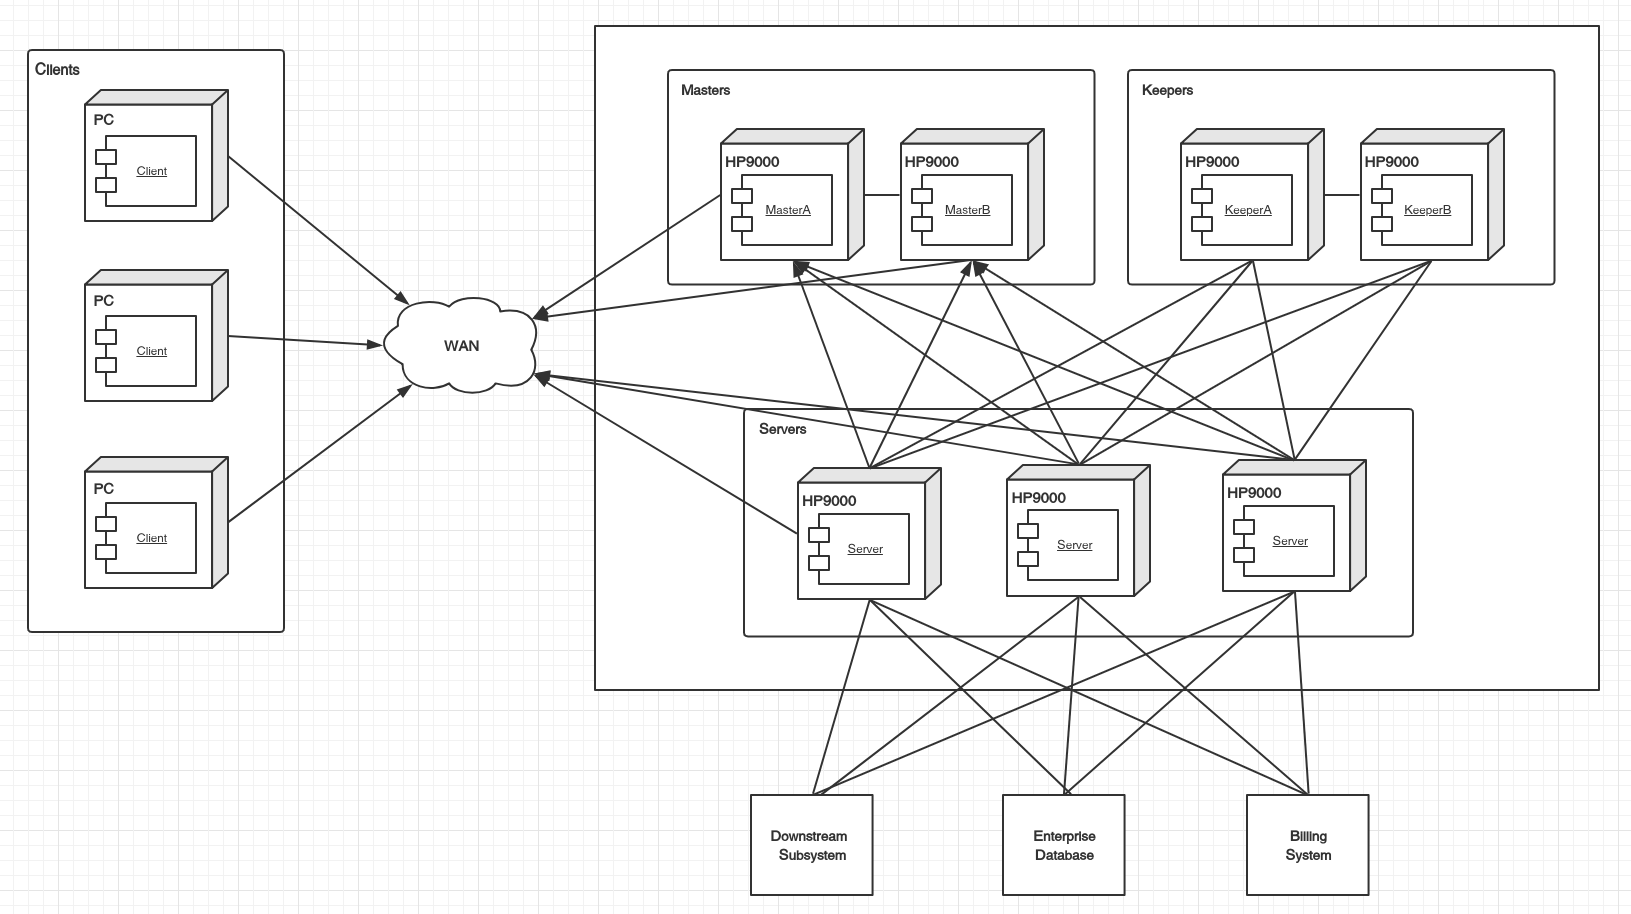
\includegraphics[scale=0.25]{deployment1.png}
			\end{center}
			\paragraph{Section 2: The Element Catalog}
			\subparagraph{Elements and their properties}
			\begin{itemize}
			\item{Client} The element Clients are deployed in the physical nodes placed in the office, which is running on Windows 10 PC.
			\item{Master} The master node of server cluster, providing functionalities such as load balancing, service registration, and service management. The master node is deployed independently to two HP9000 servers through dual hot standby mode.
			\item{Server} Server is the node that provides business service processing capabilities in the server cluster and is deployed on multiple HP9000 servers. These server nodes are redundant nodes and provide the same business service processing functionality.
			\item{Keeper} Distributed service coordination node, providing distributed locks and service processing context storage for server node cluster.
			\end{itemize}
			\subparagraph{Relations and their properties}
			\begin{itemize}
			\item{Client} Processing the business by communicating
			 with the server cluster through the WAN
			\item{Master} Clients will request the Master to obtain services list and Master will return a suitable services list for Clients based on the current load.
			\item{Server} The actual request of Clients is directly performed with the Server, not Master; when the Server node starts, it will register the service with the Master node, keep connection with Master node during the normal service provision, and report the load status and other information to Master node; During the business processing, the Server nodes will communicate with other systems outside (including downstream subsystems, enterprise databases, billing systems, NOSS, etc.) when necessary.
			\item{Keeper} The Server node will obtain or release the lock from Keeper; when involving business interruption or recovery, the Server node will also save or obtain the business context from Keeper.
			\end{itemize}
			\subparagraph{Element interfaces}
			\begin{itemize}
			\item{Client} End user interaction interface
			\item{Master} Service registration interface; service list acquisition interface; load information collection interface
			\item{Server} All business function interface; synchronous/asynchronous communication interface with external system
			\item{Keeper} Read/Write interface of business context information; lock service interface
			\end{itemize}
			\subparagraph{Element behavior}
			\begin{itemize}
			\item{Client} Respond to end user interaction
			\item{Master} In response to the Client's service list obtaining request, Master will generate an appropriate service list and returns according to the current cluster load situation and the predefined load balancing policy; Collecting periodic load information reports from Server nodes; If load information report of a Server node is not received within the certain period, the Server node is considered to be failed, and will be removed from the service list; Accept and process service registration requests from eht new Server nodes			
			\item{Server} Respond to Clients' business requests; Periodically processing asynchronous responses from external systems  in the message queue; When Clients request to interrupt the current business, the Server will save the current business context in Keeper, and when Clients request to restore the current business, Server obtains the stored context information from the Keeper and returns it; For each Client's business, Server will request Keeper to lock or release lock of related system resources 			
			\item{Keeper} Response to Servers' lock service request according to the current resources lock situation; Response to Servers' context read and write requests			
			\end{itemize}
			\paragraph{Section 3: Context Diagram}
			\begin{center}
			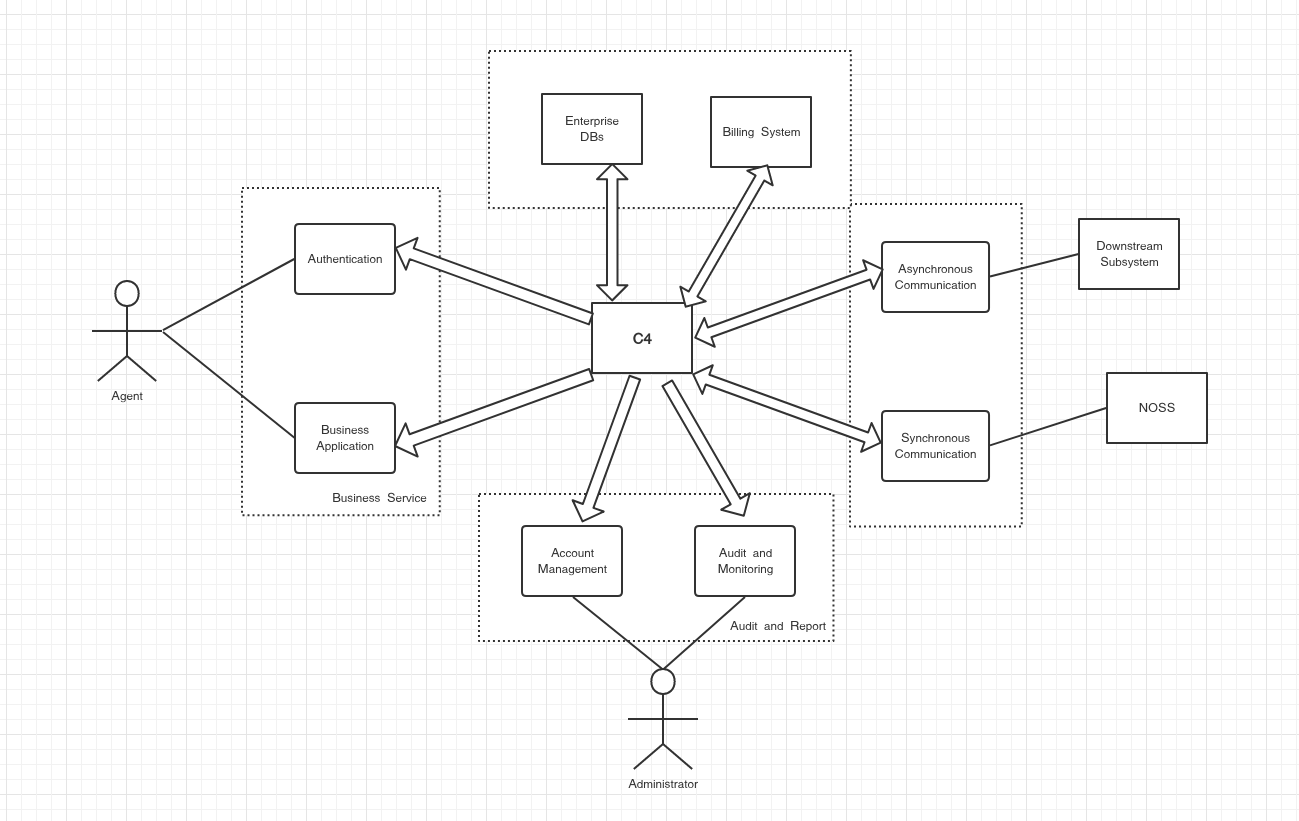
\includegraphics[scale=0.3]{deployment2.png}
			\end{center}
			\paragraph{Section 4: Variability Guide}
			With the growth of business in the future, the number of office agents will increase, so the number of Client nodes that need to be deployed will also increase. In order to cope with the larger work load, the Server nodes will introduce more deployment nodes accordingly.
			\paragraph{Section 5: Rationale}
			Because of the high availability requirement of the system, the system needs to respond to the failure of the Server nodes through redundancy (including Client nodes and Server nodes). Secondly, in order to coordinate the management of distributed Server node cluster, we introduce the Master node to implement service registration and service management, and in order to solve the single point failure, Master nodes adopt the scheme of dual-system hot standby and physical node independent deployment.\\
			Since the concurrent tasks in the normal service processing may cause problems such as configuration requests conflicts and system resource conflicts, and the requirement of saving the interrupted business context, the system needs to ensure data consistency under distributed clusters.Therefore, we introduces Keeper to provide the functionality of distributed lock, and in order to solve the problem of single point failure, Keeper nodes also adopt cluster mode and independent physical node deployment.
			
	\subsection{Mapping Between Views}
	TODO

	\subsection{Rationale}
	Explain what decision we have made in our views.

	\subsection{Directory}


	\section{Personal Remarks}
	\subsection{Statement of ...}
	\subsection{Statement of ...}
	\subsection{Statement of ...}
	\subsection{Statement of ...}
\end{document}